\documentclass[11pt]{article}
\usepackage[hmargin=1in,vmargin=1in]{geometry}
\usepackage{xcolor}
\usepackage{amsmath,amssymb,amsfonts,url,sectsty,framed,tcolorbox,framed,graphicx}
\newcommand{\pf}{{\bf Proof: }}
\newtheorem{theorem}{Theorem}
\newtheorem{lemma}{Lemma}
\newtheorem{proposition}{Proposition}
\newtheorem{definition}{Definition}
\newtheorem{remark}{Remark}
\newcommand{\qed}{\hfill \rule{2mm}{2mm}}

\begin{document}
\noindent
\rule{\textwidth}{1pt}
\begin{center}
{\bf [CS304] Introduction to Cryptography and Network Security}
\end{center}
Course Instructor: Dr. Dibyendu Roy \hfill Winter 2022-2023\\
Scribed by: Srushti Rathva (202051183) \hfill Lecture (Week 5)
\\
\rule{\textwidth}{1pt}

\section*{Group}
$\alpha \in G$ \\
$ \alpha^{0}, \alpha^{1}, \alpha^{2}, \alpha^{3} \in G $ \\
For any $ b \in G $, if $\exists$ $i \geq 0$ such that $b = \alpha^{i}$, then $\alpha$ is called \textbf{generator of (G,*)}. \\
(G,*) = $< \alpha >$ 

\subsection*{Cyclic Group}
For given (G,*), \\
$|G|$ = finite \\
$a^{m} = e$ \\
$ O(a) = m$ \\
H = \{$ a^{0}, a^{1}, a^{2} ... a^{m-1} $ \} \\ \\
A group G is called cyclic if satisfies following conditions : \\
1. $ H \subseteq G$ \\
2. H is group under * \\

\section*{Lagrange's Theorem}
If G is a finite group and H is subgroup of G then $|H|$ divides $|G|$. \\
For given (G,*), \\
$|G|$ = finite \\
$a \in G $ \\
$O(a)$ $|$ $|G|$ \\
H = \{$ a^{0}, a^{1}, a^{2} ... a^{O(a)-1} $ \} \\
Here, H is a subgroup of G. \\ \\
From Lagrange's Theorem, \\
$|H|$ $|$ $|G|$ \\
$O(a)$ $|$ $|G|$ \\ \\
If order of $a \in G$ is t then,\\
$O(a^{k}) = \frac{t}{gcd(t,k)}$ \\

\section*{Ring}
It $R(+_{R},*_{R})$ consists of one set R with two binary operations arbitrarily denoted by $+{R}$ and $*_{R}$ on R, following with properties : \\
1. (R,$+_{R}$) is an abelian with identity element $0_{R}$. \\
2. $*_{R}$ is associate. \\
3. $\exists$ an identity element for $*_{R}$. \\
4. $*{R}$ is distributive over $+{R}$. \\

\subsection*{Commutative Ring}
A ring $R(+_{R},*_{R})$ is called commutative if, \\
$a *_{R} b$ = $b *_{R} a$ , $\forall$ a,b $\in$ R

\subsection*{Unit or Invertible Element}
An element is $a$ of a ring $R$ is called \textbf{unit element} or \textbf{invertible element} if $\exists$ $ b \in R$ such that \\
$a*_{R}b$ = $1_{R}$ 
\\ \\
The set of units in a ring $R$ forms a group under multiplication operation.\\
This is called as \textbf{group of units of R}.

\section*{Field}
It consists of one set $F(+,*)$ with two binary operations satisfying following properties : \\ 
1. (F,+) is an abelian group. \\
2. If $0_{F}$ is additive identity element then $(F\setminus \{0_{F}\},*)$ is commutative group. \\
3. $*$ is distributive over $+$. \\

\section*{Field Extension}
Suppose $K_{2}$ is field  with $+$ and $*$. \\
Suppose $k_{1} \subseteq k_{2}$ is closed under both these operations such that $k_{1}$ itself is a field with the restriction of $+$ and $*$ to the set $k_{1}$. \\
$k_{1}$ is called \textbf{subfield} of $k_{2}$ and $k_{1}$ is called \textbf{field extension} of $k_{2}$. \\

\section*{Polynomial Ring}
$(F[x],+,*)$ is called polynomial ring if it satisfies following properties : \\
1. (F[x],+) is an abelian group. \\
2. $*$ is associative. \\
3. $*$ is distributive over $+$. \\
4. 1 is multiplicative identity. \\ \\
$+$ : polynomial addition \\
$*$ : polynomial multiplication \\ \\
$P_{1}(x) \in F[x] $ \\
$P_{2}(x) \in F[x] $ \\ \\
$P_{1}(x) + P_{2}(x) \in F[x] $ \\
$P_{1}(x) * P_{2}(x) \in F[x] $ 

\subsection*{Irreducibe Polynomial}
A polynomial $P(x) \in F[x]$ of degree n$\geq$1 is called \textbf{irreducible} if it cannot be written in the form of $P_{1}(x) * P_{2}(x)$, with $P_{1}(x)$ , $P_{2}(x)$ $\in$ F[x] and degree of $P_{1}(x) * P_{2}(x) \geq 1$. \\
\\
For example, \\
$x^{2}+1$ = $(x+1)(x+1)$ = $x^{2} + (1+_{2}1)x + 1$ = $x^{2}+1$ 

\subsection*{Irreducibility and Field}
$I$ = $<p(x)>$ = $\{q(x)*p(x) | q(x) \in F[x]\}$ , where I $\rightarrow$ Ideal generated by $p(x)$ \\ \\
$p(x), q(x) \in F[x]$ \\
deg(r(x)) $<$ deg(p(x)) \\ \\
$F[x] / <p(x)>$ $\rightarrow$ $g(x) \in F[x]$ \\
$q(x) = d(x)*p(x) + r(x)$ \\
$r(x) \in F[x] / <p(x)>$ \\ \\
If p(x) is irreducible polynomial then $(F[x] / <p(x)>,+,*)$ becomes field. \\
\\
For example, \\
$x^{2}+x+1 \in F[x]$, $F=\{0,1\}$ \\
Here, $p(x)$ = $x^{2}+x+1$ is irreducible. \\
$ F[x] / <x^{2}+x+1>$ \\
$q(x) = d(x)*p(x) + r(x)$ \\
deg(r(x)) $<$ 2 \\ \\
Let's assume $\alpha$ is root of $p(x)$ then, \\
$\alpha^{2}+\alpha+1 = 0$ \\
$\alpha^{2} = \alpha+1$ \\ \\
We can generate all polynomials using $\alpha$. \\
\{$ 0, \alpha^{0}=1, \alpha^{1}, \alpha^{2} = \alpha + 1 ...$ so on\} \\
Hence, $x^{2}+x+1$ is called a \textbf{primitive polynomial}.\\

\section*{Advanced Encryption Standard (AES)}
Winner of competition was Rijndael and winning implementation was named AES. \\
It is iterated block cipher and It is based on Substitution Permutation Network (SPN). \\

\subsection*{AES - 128}
1. Block Size = 128 bits \\
2. No. of Rounds = 10 \\
3. Secret key Size = 128 bits

\subsection*{AES - 192}
1. Block Size = 128 bits \\
2. No. of Rounds = 12 \\
3. Secret key Size = 192 bits

\subsection*{AES - 256}
1. Block Size = 128 bits \\
2. No. of Rounds = 14 \\
3. Secret key Size = 256 bits \\
\\
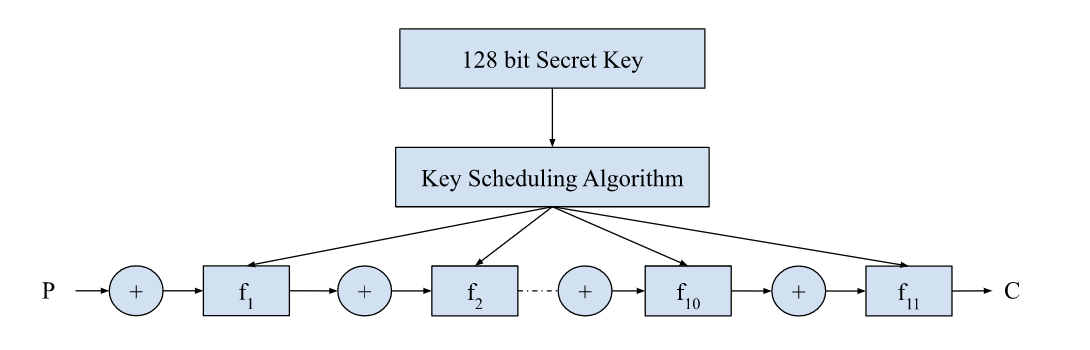
\includegraphics[width=500pt]{p1.png}
\end{document}
